\documentclass{standalone}
\usepackage{tikz}
\usepackage{graphicx}
\usetikzlibrary{arrows.meta}

\begin{document}
\begin{tikzpicture}
    %\draw[white] (0,0) rectangle (29.7,21);
    \node[anchor=south west,inner sep=0] at (0,0)
    {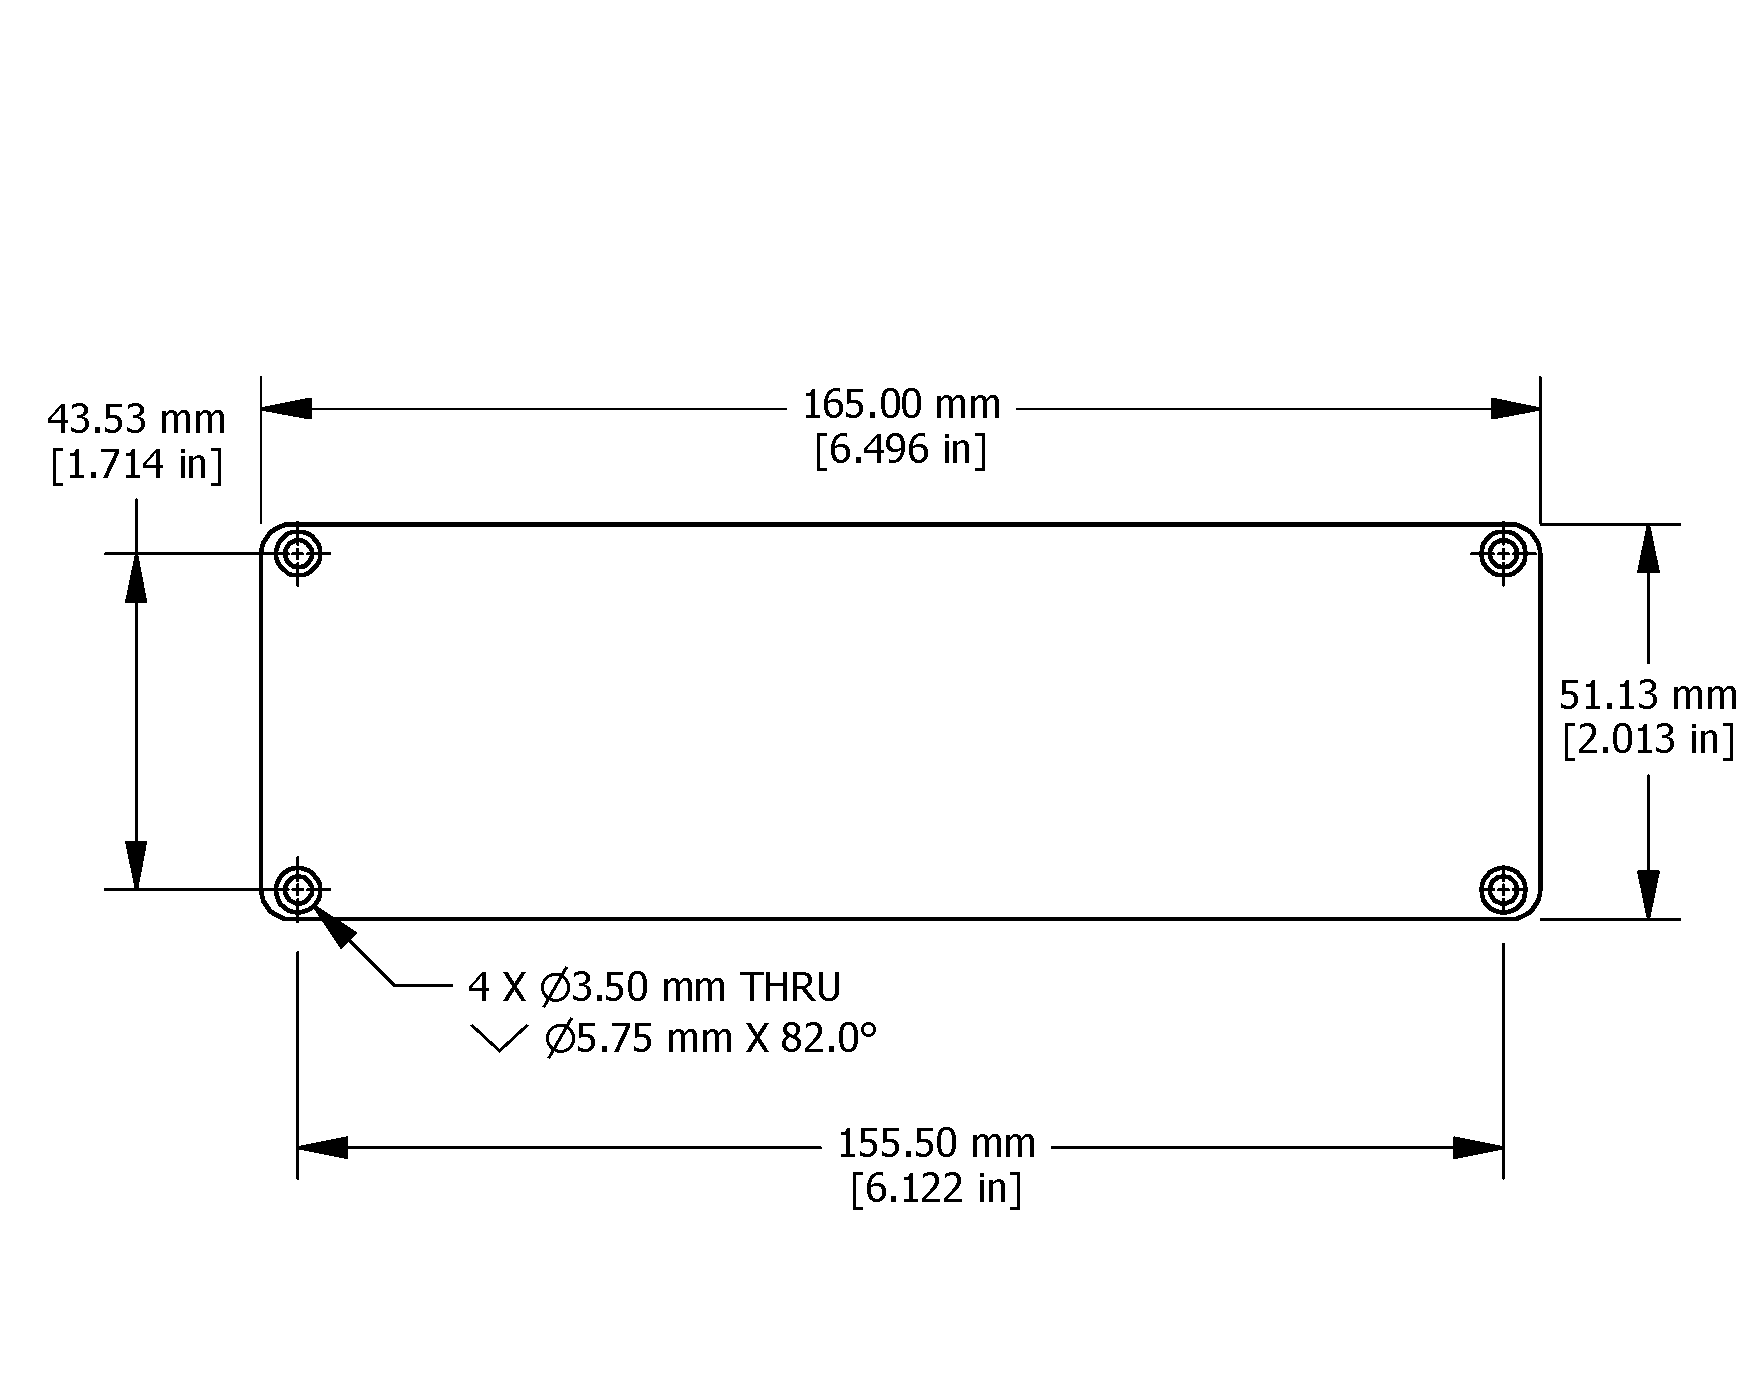
\includegraphics[width=297mm]{images/faceplate.pdf}};

    % REFERENCE LINE HORIZONTAL
    % total width: 165 mm
    % length arrow: 217.2 mm
    %\draw[|Stealth-{Stealth}|,ultra thick] (4.4,16) -- (26.12,16);


    % REFERENCE LINE VERTICAL
    % total height: 51.13 mm
    % length arrow: 67.5 mm
    %\draw[|Stealth-{Stealth}|,ultra thick] (27,14.5) -- (27,7.75);


    % line from right edge of face plate to right edge of rocker switch opening
    % 12 mm from right edge: 15.8 mm in coordinate system
    \draw[Stealth-Stealth,thick] (26.12,11.125) -- (24.54,11.125);
    \node at (25.33,11.5) {\large{12.0mm}};
    \draw[Stealth-Stealth,thick] (26.12-1.58-1.699/2,14.5) -- (26.12-1.58-1.699/2,14.5-6.75/2+2.527/2);
    \node at (22.7,13.5) {\large{16.0mm}};
    % rectangle size: 12.9 mm x 19.2 mm: 16.99 mm x 25.27 mm in drawing
    \fill[lightgray] (24.54,11.125-2.527/2) rectangle (24.54-1.699,11.125+2.527/2);
    \draw[thick] (24.54,11.125-2.527/2) rectangle (24.54-1.699,11.125+2.527/2);

    % horizontal arrow inside rectangle for rocker switch
    \draw[Stealth-Stealth,thick] (24.54,11.125) -- (24.54-1.699,11.125);
    \node at (24.54-1.699/2,11.5) {\large{12.9mm}};

    % vertical arrow for rocker switch opening
    \draw[-,thick] (24.54-1.699,11.125-2.527/2) -- (24.54-1.699-1,11.125-2.527/2);
    \draw[-,thick] (24.54-1.699,11.125+2.527/2) -- (24.54-1.699-1,11.125+2.527/2);
    \draw[Stealth-Stealth,thick] (24.54-1.699-0.5,11.125-2.527/2) -- (24.54-1.699-0.5,11.125+2.527/2);
    \node at (24.54-1.699-1.3,11.125) {\large{19.2mm}};

    % LCD bezel
    % actual measurements: (85.5+-0.2)mm x (28.5+-0.2)mm
    % drawing dimensions: 112.55 mm x 37.52 mm
    % distance to left edge: 15 mm real, 19.7454 mm in drawing
    \fill[lightgray] (4.4+1.975,11.125-3.752/2) rectangle (4.4+1.975+11.255,11.125+3.752/2);
    \draw[thick] (4.4+1.975,11.125-3.752/2) rectangle (4.4+1.975+11.255,11.125+3.752/2);
    \draw[Stealth-Stealth,thick] (4.4,11.125) -- (4.4+1.975,11.125);
    \node at (4.4+1.975/2,11.5) {\large{15mm}};
    \draw[Stealth-Stealth,thick] (4.4+1.975,8.5) -- (4.4+1.975+11.255,8.5);
    \node at (4.4+1.975+11.255/2,8.75) {\large{86mm}};
    \draw[-,thick] (4.4+1.975,11.125) -- (4.4+1.975,8.25);
    \draw[-,thick] (4.4+1.975+11.255,11.125) -- (4.4+1.975+11.255,8.25);

    \draw[Stealth-Stealth,thick] (4.4+1.975+11.255/2,11.125+3.752/2) -- (4.4+1.975+11.255/2,11.125-3.752/2);
    \node at (4.4+11.255/2+1.25,14.5-6.75/2) {\large{29mm}};

    %\draw[-,thick] (4.4+1.975+11.255,11.125-3.752/2) -- (4.4+1.975+11.255+1,11.125-3.752/2);
    %\draw[-,thick] (4.4+1.975+11.255,11.125+3.752/2) -- (4.4+1.975+11.255+1,11.125+3.752/2);

    \draw[Stealth-Stealth,thick] (4.4+1.975+11.255/2,11.125+3.752/2) -- (4.4+1.975+11.255/2,14.5);
    \node at (4.4+11.255/2+1.2,14.5-6.75/2+3.752/2+6.75/4-3.752/4) {\large{11.1mm}};
    %\draw[thick] (24.54,11.125-2.527/2) rectangle (24.54-1.699,11.125+2.527/2);


    % marking for thingy hole
    % distance to vertical center of hole: 120.55 mm
    % on drawing: 158.69 mm
    \draw[Stealth-Stealth,thick] (4.4,15) -- (4.4+15.69,15);
    \draw[-,thick] (4.4+15.69,15.5) -- (4.4+15.69,8.75);
    \draw[-,thick] (4.4+15.69,11.125-0.2) -- (4.4+15.69,11.125+0.2);
    \node at (4.4+15.69/2,15.3) {\large{120.6mm}};

    \draw[Stealth-Stealth,thick] (4.4+15.69,14.5) -- (4.4+15.69,11.125);
    \draw[-,ultra thick] (4.4+15.69-0.2,11.125) -- (4.4+15.69+0.2,11.125);
    \draw[-,thick] (4.4+15.69-0.2,11.125) -- (4.4+15.69+0.2,11.125);
    \node at (4.4+14.7,11.125+1.6875) {\large{25.565mm}};



\end{tikzpicture}
\end{document}
